\documentclass[12pt]{article}
\usepackage[margin=3cm]{geometry}
\usepackage{graphicx}
\usepackage{pgfplots}
\pgfplotsset{width=10cm,compat=1.9}

\begin{document}

\title{Relatório 1º Projeto ASA 2023/2024}
\author{Grupo: TP048 \\ Aluno: Gabriel Silva (102637)}
\date{}
\maketitle

\section{Descrição do Problema e da Solução}

\textbf{Descrição do problema:} Dada uma chapa de mármore, calcular o valor máximo que pode ser obtido a partir da mesma cortando-a em peças correspondentes às dimensões solicitadas pelos clientes.

\textbf{Descrição da solução:} Cria-se o vetor bidimensional dp, de dimensões $(X + 1) \times (Y + 1)$, que guardará os valores máximos para cada subproblema, todos inicializados a 0. Ao ler o input em relação às peças para serem produzidas, verifica-se para cada uma se "cabe" na chapa de mármore, com ou sem rotação, e atualiza-se o valor correspondente no vetor. Iterando, usando nested loops, sobre todos os subproblemas $(i, j)$ que representam as dimensões da chapa de mármore restante, são explorados todos os cortes possíveis, verticais ou horizontais, e atualizados os valores no vetor. É feita uma abordagem de programação dinâmica bottom-up.

\section{Análise Teórica}

\begin{itemize}
    \item Leitura dos dados de entrada (depende do número de peças a serem produzidas): $O(n)$
    \item Inicializar o vetor bidimensional de dimensão $(X + 1) \times (Y + 1)$: $O(X \times Y)$
    \item Loop de programação dinâmica (3 nested loops): $O(X^2 \times Y^2)$
    \item Apresentação dos dados: $O(1)$
\end{itemize}

Complexidade global da solução: $O(X^2 \times Y^2)$

\section{Avaliação Experimental dos Resultados}

\begin{table}[h]
    \centering
    \begin{tabular}{|c|c|}
        \hline
        \textbf{Tamanho} & \textbf{Tempo} \\
        \hline
        30000 & 0.005 \\
        60000 & 0.009 \\
        120000 & 0.016 \\
        180000 & 0.024 \\
        270000 & 0.041 \\
        360000 & 0.062 \\
        480000 & 0.090 \\
        600000 & 0.129 \\
        750000 & 0.172 \\
        900000 & 0.228 \\
        1080000 & 0.296 \\
        1260000 & 0.375 \\
        1470000 & 0.466 \\
        1680000 & 0.571 \\
        1920000 & 0.695 \\
        2160000 & 0.829 \\
        2430000 & 0.992 \\
        2700000 & 1.164 \\
        3000000 & 1.370 \\
        3300000 & 1.565 \\
        3630000 & 1.861 \\
        3960000 & 2.192 \\
        4320000 & 2.392 \\
        4680000 & 2.704 \\
        5070000 & 2.995 \\
        \hline
    \end{tabular}
    \caption{Tamanho instâncias (X * Y * N) e o Tempo (segundos)}
\end{table}

\begin{figure}[h]
    \centering
    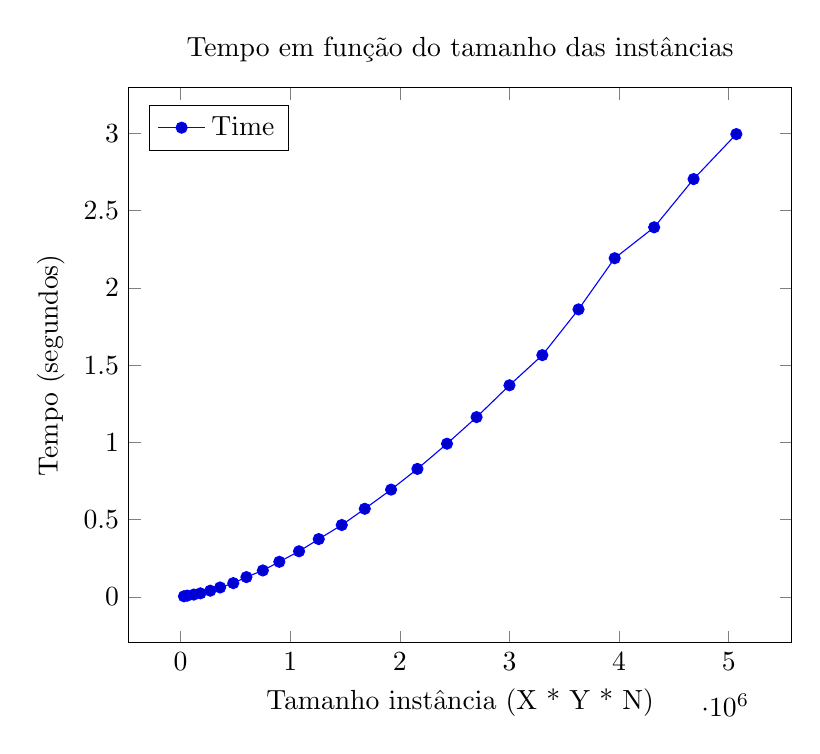
\begin{tikzpicture}
        \begin{axis}[
            xlabel={Tamanho instância (X * Y * N)},
            ylabel={Tempo (segundos)},
            title={Tempo em função do tamanho das instâncias},
            legend pos=north west,
        ]
            \addplot table[x=Size, y=Time, col sep=semicolon] {
                Size;Time
                30000;0.005
                60000;0.009
                120000;0.016
                180000;0.024
                270000;0.041
                360000;0.062
                480000;0.090
                600000;0.129
                750000;0.172
                900000;0.228
                1080000;0.296
                1260000;0.375
                1470000;0.466
                1680000;0.571
                1920000;0.695
                2160000;0.829
                2430000;0.992
                2700000;1.164
                3000000;1.370
                3300000;1.565
                3630000;1.861
                3960000;2.192
                4320000;2.392
                4680000;2.704
                5070000;2.995
            };
            \legend{Time}
        \end{axis}
    \end{tikzpicture}
\end{figure}

\end{document}
